\documentclass[10pt,a4paper]{report}
\usepackage{listings}
\usepackage{color}
\definecolor{dkgreen}{rgb}{0,0.6,0}
\definecolor{gray}{rgb}{0.5,0.5,0.5}
\definecolor{mauve}{rgb}{0.58,0,0.82}
\lstset{frame=tb,
  language=Java,
  aboveskip=3mm,
  belowskip=3mm,
  showstringspaces=false,
  columns=flexible,
  basicstyle={\small\ttfamily},
  numbers=none,
  numberstyle=\tiny\color{gray},
  keywordstyle=\color{blue},
  commentstyle=\color{dkgreen},
  stringstyle=\color{mauve},
  breaklines=true,
  breakatwhitespace=true,    
  tabsize=3
}
\usepackage[utf8]{inputenc}
\usepackage{amsmath}
\usepackage{amsfonts}
\usepackage{amssymb}
\usepackage{graphicx}
\usepackage{lmodern}
\usepackage[left=2cm,right=2cm,top=2cm,bottom=2cm]{geometry}
\begin{document}
\author{Yapi Donatien Achou}
\title{Cable problem with 2 P1 elements}
\maketitle
\section{Setting up the problem}
Consider the problem
\begin{equation}\label{main}
u^{\prime\prime} = 1 
\end{equation}
with Dirichlet boundary condition

\begin{equation} \label{bc}
u(0) = u(1)= 0
\end{equation}
let V be given by 

\begin{equation}
V = span\{\varphi_{0}\cdots\varphi_{N}\} \nonumber
\end{equation}
where $\varphi_{i}$ are the Lagrange elements of order 1.
\section{Variational formulation}
The variational formulation of (\ref{main}, \ref{bc}) is: Find $u\in V$ such that :

\begin{equation}\label{var}
-\int_{0}^{1} u^{\prime}v^{\prime} \mathrm{d}x = \int_{0}^{1} v \mathrm{d}x \quad \forall v\in V.
\end{equation}

with 
\begin{equation}
a(u,v) = -\int_{0}^{1} u^{\prime}v^{\prime} \mathrm{d}x\nonumber
\end{equation}

\begin{equation}
L(v) = \int_{0}^{1} v \mathrm{d}x\nonumber
\end{equation}
\section{Finite element solution}
$u,v \in V$ mean that $u$ and $v$ can be written as the linear combination of $\varphi_{i}$:

\begin{equation}\label{u}
u = \sum_{i = 0}^{N}c_{i}{\varphi_{i}}
\end{equation}

\begin{equation}\label{v}
v = \varphi_{j}
\end{equation}
Inserting (\ref{u}, \ref{v}) in \ref{var} gives:
\begin{equation}
-\int_{0}^{1} \varphi_{i}^{\prime}\varphi_{i}^{\prime} \mathrm{d}x\sum_{i = 0}^{N}c_{i} = \int_{0}^{1}\varphi_{j} \mathrm{d}x 
\end{equation}
where the stiffness matrix $K$ and the load matrix $b$ are respectively given by:

\begin{equation}
K_{ij} = -\int_{0}^{1} \varphi_{i}^{\prime}\varphi_{i}^{\prime} \mathrm{d}x \nonumber
\end{equation}

\begin{equation}
b_{j} = \int_{0}^{1}\varphi_{j} \mathrm{d}x \nonumber
\end{equation}

The basis function $\phi_{i}$ and their derivatives are given by:

\[
 \varphi_{i}(x) =
  \begin{cases}
   0 & \text{if } x < x_{i-1} \\
   \frac{x-x_{i-1}}{h}       & \text{if } x_{i-1} \leq  x < x_{i}\\
   1-\frac{x-x_{i}}{h}      & \text{if } x_{i} \leq  x < x_{i+1}\\
   0     & \text{if }   x \ge x_{i+1}
  \end{cases}
\]

\[
 \varphi_{i}^{\prime}(x) =
  \begin{cases}
   0 & \text{if } x < x_{i-1} \\
   \frac{1}{h}       & \text{if } x_{i-1} \leq  x < x_{i}\\
   -\frac{1}{h}      & \text{if } x_{i} \leq  x < x_{i+1}\\
   0     & \text{if }   x \ge x_{i+1}
  \end{cases}
\]

Ad we have
\begin{equation}
K_{ii} = \frac{2}{h} \nonumber
\end{equation}
\begin{equation}
K_{i,i-1} = A_{i,i+1} =-\frac{1}{h}\nonumber
\end{equation}

\begin{equation}
b_{j} =  h \nonumber
\end{equation}

with N = 1 we have
\begin{equation}
K =\frac{1}{h} \begin{bmatrix}
       2 & -1           \\
       -1& 2             
     \end{bmatrix}
\end{equation}

\begin{equation}
K^{-1} =\frac{h}{3} \begin{bmatrix}
       2 & 1           \\
       1& 2             
     \end{bmatrix}
\end{equation}

\begin{equation}
b =h \begin{bmatrix}
       1            \\
       1             
     \end{bmatrix}
\end{equation}

And solving the system
\begin{equation}
Kc = b \rightarrow c = K^{-1}b \nonumber
\end{equation}

\begin{equation}
c_{0} = c_{1} = \frac{h^{2}}{3}\nonumber
\end{equation}

\begin{equation}
u(x) = \frac{h^{2}}{3}\varphi_{0}+\frac{h^{2}}{3}\varphi_{1} \nonumber
\end{equation}

\section{Solution with fenics for N = 60}

\begin{lstlisting}
from dolfin import *

#define mesh
mesh = UnitIntervalMesh(60)
V = FunctionSpace(mesh,'Lagrange',1)

# set Dirichlet boundary condition
u0 = Expression('0.0')
def u0_boundary(x,on_boundary):
    return on_boundary

bc = DirichletBC(V,u0,u0_boundary)

# varional formulation
u = TrialFunction(V)
v = TestFunction(V)
f = Constant(1)
a = -inner(grad(u),grad(v))*dx
L = f*v*dx

# solution of the variatiobal problem
u = Function(V)
solve(a==L,u,bc)

#plot solution
plot(u)

# view solution
interactive()
\end{lstlisting}

\begin{figure}[H]
  \caption{Deflection of the cable with finite element for N = 60}
  \centering
    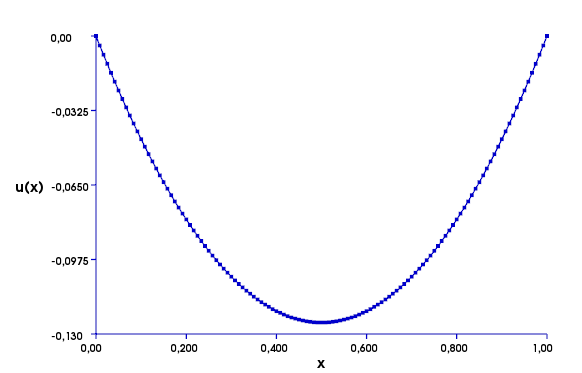
\includegraphics[width=0.5\textwidth]{cable.png}
\end{figure}

\end{document}